\chapter{Victor's Money Game}

This chapter follows a School of Hard Knocks interview with Victor, curated for the LazyEarn track by LazyingArt LLC. The source is an interview rather than a blackboard lecture, so the mathematics here is practical arithmetic: claims about scale, target decomposition, repeated exposure, reinvestment, and time. We will keep the numbers in their proper status as interview claims, then turn only the transcript-supported mechanisms into equations, tables, and small diagrams.

\section{Opening Claim: From Zero to Eight Figures}

The interview begins by setting a gap before it explains a method. Victor is introduced as a young Houston entrepreneur who, in the interview's framing, moved from zero dollars at 19 to a net worth over ten million dollars by 26. Let \(N_a\) denote the claimed net worth at age \(a\). The opening contrast is

\begin{equation}
N_{19} \approx 0,
\qquad
N_{26} > 10{,}000{,}000.
\end{equation}

This notation is only a bookkeeping device for the transcript. It is not an audited balance sheet. Its purpose is to preserve the size of the claim before we ask what mechanism is supposed to explain it.

The next number is a current-year flow. When James asks about the most money Victor has made in a single year, Victor says that halfway through the year he is at six million. If \(R_{\text{half}}\) is the amount reached halfway through the year, then the transcript gives

\begin{equation}
R_{\text{half}} \approx 6{,}000{,}000.
\end{equation}

The title points to twelve million a year. That number is best treated as an annualized run-rate inference from the halfway claim:

\begin{equation}
R_{\text{annualized}}
\approx 2R_{\text{half}}
\approx 2 \times 6{,}000{,}000
= 12{,}000{,}000.
\end{equation}

So the opening does two things at once. It gives the reader the drama of the jump, and it teaches the first rule of these notes: keep the concrete numbers, but keep their evidentiary status visible.

\section{The First Mechanism: Weekly Drops and Attention}

Once the headline is established, the interview moves backward to the first business. Victor says he started at 19 with a clothing brand, an e-commerce apparel business. James then asks the natural competitive question: many people try to make apparel brands, so what made this one stand out?

Victor's answer is cadence. He does not begin with a theory of brand identity or a perfect launch. He says he dropped clothes every week, good or bad, with or without immediate sales. The point was to keep appearing in front of people while other creators held a project for months, trying to perfect it.

A compact way to write the mechanism is

\begin{equation}
\text{weekly drops}
+
\text{repeated exposure}
+
\text{market feedback}
\longrightarrow
\text{attention advantage}.
\end{equation}

The arrow is not a guaranteed causal law. It is an editorial shorthand for Victor's claim: in a crowded social-media market, repetition changes the probability of being noticed.

\subsection{Question \& Answer}

\paragraph{Question.}
Why might imperfect weekly drops beat a polished six-month launch?

\paragraph{Answer.}
Because the market is not only evaluating product quality; it is also allocating attention. Victor's point is that people are not waiting six months for a beginner's perfect project. A weekly drop creates contact, feedback, and familiarity. The brand becomes part of the audience's normal feed before it becomes part of the audience's buying habit.

\begin{figure}[h]
\centering
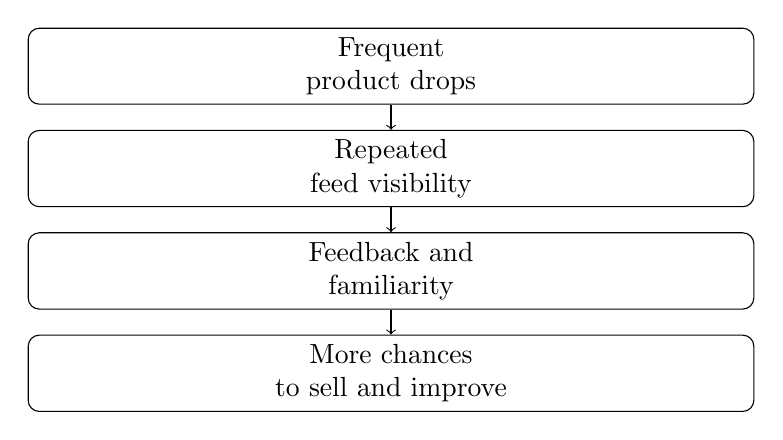
\begin{tikzpicture}
\node[draw, rounded corners, align=center, minimum width=0.76\linewidth] (a) at (0,0) {Frequent\\product drops};
\node[draw, rounded corners, align=center, minimum width=0.76\linewidth] (b) at (0,-1.30) {Repeated\\feed visibility};
\node[draw, rounded corners, align=center, minimum width=0.76\linewidth] (c) at (0,-2.60) {Feedback and\\familiarity};
\node[draw, rounded corners, align=center, minimum width=0.76\linewidth] (d) at (0,-3.90) {More chances\\to sell and improve};
\draw[->] (a) -- (b);
\draw[->] (b) -- (c);
\draw[->] (c) -- (d);
\end{tikzpicture}
\caption{A transcript-grounded attention cadence: repeated releases create repeated market contact.}
\end{figure}

\section{Making a Million Smaller}

The interview next turns from getting attention to scaling. James asks how Victor turned six figures into seven figures. Victor's answer is the arithmetic center of the conversation: money is a game of numbers, and the million-dollar figure overwhelms people because they see it as one object.

The transcript compresses the wording, but the intended calculation is clear enough to state with a caveat:

\begin{align}
10{,}000 \times 10 &= 100{,}000, \\
100{,}000 \times 10 &= 1{,}000{,}000.
\end{align}

Victor also uses a doubling image in the opening montage: one car can become two, two can become four, and four can become a fleet. As a metaphor, that is

\begin{equation}
1 \longrightarrow 2 \longrightarrow 4 \longrightarrow \text{fleet}.
\end{equation}

We should not overread this as a formal exponential-growth model. In context, it is a way of saying that the operator should think in repeated, compounding moves rather than in one heroic leap.

\begin{table}[h]
\centering
\begin{tabular}{c|c|c}
Milestone & Repeated unit & Count \\
\hline
\(100{,}000\) & \(10{,}000\) & \(10\) \\
\(1{,}000{,}000\) & \(100{,}000\) & \(10\) \\
\end{tabular}
\caption{The money ladder, normalized from Victor's compressed spoken arithmetic.}
\end{table}

\subsection{Question \& Answer}

\paragraph{Question.}
How does breaking the target into repeated units change the operator's behavior?

\paragraph{Answer.}
It changes the target from a symbol of intimidation into a sequence of actions. A million dollars is psychologically large. Ten repetitions of a smaller commercial unit can be tracked, repeated, and improved. The arithmetic does not make the work easy; it makes the work addressable.

A worked version of the decomposition is

\begin{align}
G &= 1{,}000{,}000, \\
G &= 10 \times 100{,}000, \\
100{,}000 &= 10 \times 10{,}000, \\
G &= 10 \times (10 \times 10{,}000).
\end{align}

The conclusion is not merely \(G=1{,}000{,}000\). The conclusion is that the million-dollar goal has been rewritten as nested repetition. The unit of thought has changed from the whole mountain to the next climbable ledge.

\section{Bootstrapping and the Daily Update}

After the number ladder, Victor immediately returns to execution. He says that with team or no team, he did not use ads or a budget to propel the work. He describes the path as bootstrapping and showing up in the field every day.

This is where the arithmetic needs an operating update rule. Let \(A_t\) denote accumulated market position at time \(t\): audience awareness, product feedback, confidence, and practical learning. Then a cautious reconstruction of the daily logic is

\begin{equation}
A_{t+1}
=
A_t
+
\Delta_{\text{visibility}}
+
\Delta_{\text{learning}}.
\end{equation}

Here \(A_t\) is not cash, and the deltas are not measured variables in the transcript. They are a clean way to preserve the meaning of Victor's word ``consistency.'' If nothing is repeated, the decomposition in the previous section remains only arithmetic. If the operator returns to the field every day, the small increments can accumulate.

The important source-conscious point is that Victor is not proving that ads are useless. He is describing his own claim: in his case, repeated action and market presence substituted for paid amplification.

\section{Sales as Pull, Not Push}

The next question is about sales. James frames the obstacle concretely: a potential client or customer is on the fence, leaning toward no. Victor's answer is not to press harder. It is: do not push.

His reasoning is positional. Pushing too much makes the seller appear needy. Need weakens the offer. Victor's preferred position is to become good enough and visible enough that people come to him, after which access can be organized selectively.

We can write the contrast as two small mechanisms:

\begin{align}
\text{pressure selling}
&\longrightarrow
\text{seller appears needy}, \\
\text{visible demand}
&\longrightarrow
\text{selectivity}
\longrightarrow
\text{access product}.
\end{align}

The practical example comes immediately after the principle. Victor says they scaled this into an elite program, with a subscription for people who could get onto the website earlier than everyone else. The selling mechanism is therefore not just persuasion. It is the conversion of demand into structured access.

\section{Network, Rooms, and Mutual Exchange}

The interview then shifts from customers to relationships. Victor says that besides consistency, network is one of the most important things. The reason is not sentimental. It is environmental. If a person's circle is not challenging, that person may mistake a local endpoint for a true endpoint.

The next question sharpens the issue. What if someone does not know how to get into the right rooms?

\subsection{Question \& Answer}

\paragraph{Question.}
How does a beginner enter better rooms without asking for help first?

\paragraph{Answer.}
Victor's answer is to invest in oneself until one has something to offer. Do not enter with a hand out. Enter with a sharpened skill. If the other person has more money or more success but lacks a capability, the beginner can become useful by filling that missing piece.

\begin{figure}[h]
\centering
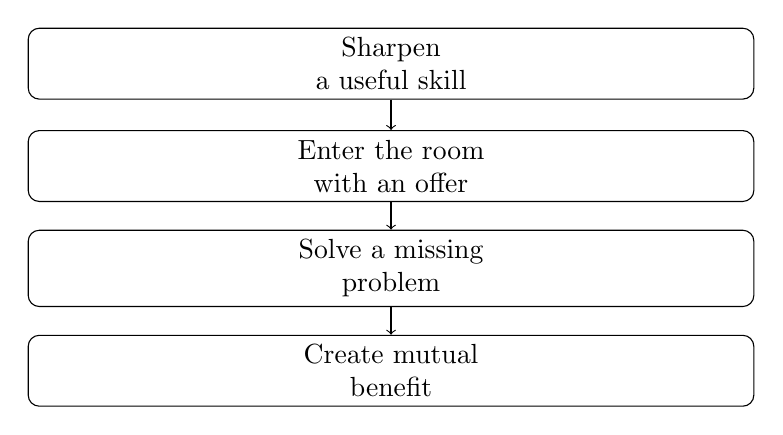
\begin{tikzpicture}
\node[draw, rounded corners, align=center, minimum width=0.76\linewidth] (a) at (0,0) {Sharpen\\a useful skill};
\node[draw, rounded corners, align=center, minimum width=0.76\linewidth] (b) at (0,-1.30) {Enter the room\\with an offer};
\node[draw, rounded corners, align=center, minimum width=0.76\linewidth] (c) at (0,-2.60) {Solve a missing\\problem};
\node[draw, rounded corners, align=center, minimum width=0.76\linewidth] (d) at (0,-3.90) {Create mutual\\benefit};
\draw[->] (a) -- (b);
\draw[->] (b) -- (c);
\draw[->] (c) -- (d);
\end{tikzpicture}
\caption{Victor's relationship mechanism: access to better rooms is framed as exchange rather than extraction.}
\end{figure}

This is one of the interview's strongest commercial distinctions. Network is not treated as vague proximity to successful people. It is treated as a matching problem between one person's missing capability and another person's developed skill.

\section{Income Becomes Assets, Time Becomes Leverage}

James then asks for the best financial advice Victor has received. Victor credits Chris Johnson and gives a phrase the transcript renders as ``get money by income.'' The wording is uncertain, but Victor defines the advice clearly: whatever money you receive, use it to buy assets that make you more money.

The wealth-conversion loop is therefore

\begin{equation}
\text{income}
\longrightarrow
\text{asset purchase}
\longrightarrow
\text{more income}
\longrightarrow
\cdots.
\end{equation}

This is a different kind of scale from the money ladder. The ladder decomposes a target. The loop changes the character of money received. A dollar can be consumed, held, or converted into a claim on future dollars. Victor's stated advice is to move income into assets that can generate more income.

\begin{figure}[h]
\centering
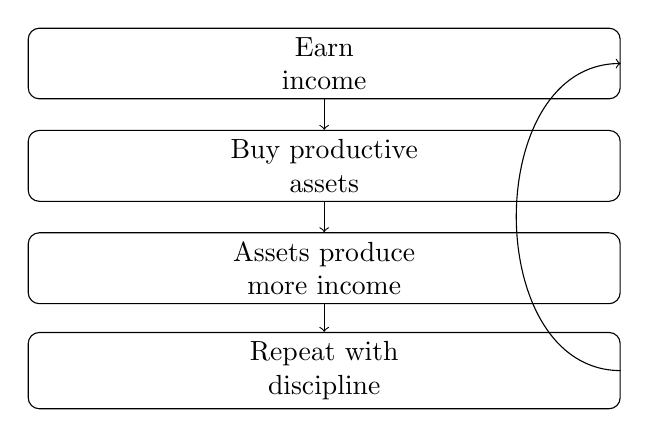
\begin{tikzpicture}
\node[draw, rounded corners, align=center, minimum width=0.62\linewidth] (a) at (0,0) {Earn\\income};
\node[draw, rounded corners, align=center, minimum width=0.62\linewidth] (b) at (0,-1.30) {Buy productive\\assets};
\node[draw, rounded corners, align=center, minimum width=0.62\linewidth] (c) at (0,-2.60) {Assets produce\\more income};
\node[draw, rounded corners, align=center, minimum width=0.62\linewidth] (d) at (0,-3.90) {Repeat with\\discipline};
\draw[->] (a) -- (b);
\draw[->] (b) -- (c);
\draw[->] (c) -- (d);
\draw[->] (d.east) .. controls (2.0,-3.90) and (2.0,0) .. (a.east);
\end{tikzpicture}
\caption{The transcript-backed reinvestment loop: received money is directed toward assets that may produce more money.}
\end{figure}

The next question turns from money to mindset. Victor says the central habit is discipline and careful selection of what one uses time on. He says time is worth more than money. In the terms of this chapter, time is the input that makes the loops possible:

\begin{equation}
\text{disciplined time}
\longrightarrow
\text{consistent action}
\longrightarrow
\text{accumulated advantage}.
\end{equation}

The temptation, as Victor describes it, is to choose the easy, fun, attractive-looking work. The compounding work is often boring, consistent, and simple. This is not a romantic statement about suffering. It is an allocation rule: scarce time should be placed where repeated action can produce accumulated advantage.

\section{Skill, Restart, and Legacy}

The final part of the interview moves quickly through skill, restart, and legacy. Asked for the most important skill for young entrepreneurs, Victor answers social media marketing. In his account, social media is the catalyst because it gives the operator a way to get in front of people.

Then comes the restart problem. If everything were taken and the bank account hit zero tomorrow, what would he do first? Victor's answer begins with network: call a friend, borrow ten thousand dollars, and run the play again. He says he would probably start a short-form service business, such as car detailing, to stack funds and keep his hands busy before moving back into digital real estate.

A source-conscious restart diagram is

\begin{equation}
0
\longrightarrow
\text{network trust}
\longrightarrow
10{,}000
\longrightarrow
\text{service cash flow}
\longrightarrow
\text{digital assets}.
\end{equation}

This should not be flattened into advice that every beginner can borrow ten thousand dollars. The more precise lesson is that, in Victor's story, network functions as part of the capital structure. It can become trust, financing, information, and opportunity.

The interview closes with reputation and purpose. Victor says he wants a wider reach and, within five years, wants to be known for helping people change their financial careers and learn business and entrepreneurship. The closing returns us to the beginning. The money game is not described only as accumulation. It is also reach, teaching, and identity after the number has been reached.

\section{Summary}

The chapter's path follows the interview's path. First comes the numerical contrast: zero dollars at 19, more than ten million in claimed net worth at 26, and six million reached halfway through the current year. Then the conversation moves into mechanisms: weekly drops, repeated attention, target decomposition, bootstrapped consistency, pull-based sales, networked exchange, reinvestment, disciplined time, social media marketing, and a restart playbook.

The mathematics is deliberately modest. A million dollars is rewritten as repeated units. Income is rewritten as a loop into assets and back into income. Attention is rewritten as repeated contact with the market. These equations are not blackboard physics; they are careful notation for the commercial mechanisms Victor describes.

The final source-conscious lesson is narrow but useful. Victor's path is not mechanically guaranteed for every reader. What the interview gives us is a sequence of operating moves: turn large goals into smaller units, repeat contact with the market, bring value into rooms, convert income into assets, and use time where repetition can compound.